\section{Einleitung}
\subsection{Einführung in die Thematik}
\blindtext\nomenclature{W3C}{World Wide Web Consortium}
\blindtext\footcite[Vgl. ][]{mswpf}

\subsection{Problemstellung und Zielsetzung}
\blindtext

\subsection{Methodischer Aufbau der Arbeit}
\blindtext

\section{Hauptteil}
\subsection{Grundlagen der Wirtschaftsinformatik}
\blindtext (vgl. Abbildung \ref{abb_bsp}).\footcite[Vgl. ][]{msdatabind}\footcite[Vgl. ][]{Atypisch}\footcite[Vgl. ][34]{Digitaloekonomie}
\blindenumerate
\Blindtext
\begin{figure} [!htb]
    \raggedright\caption{Beispiel}
    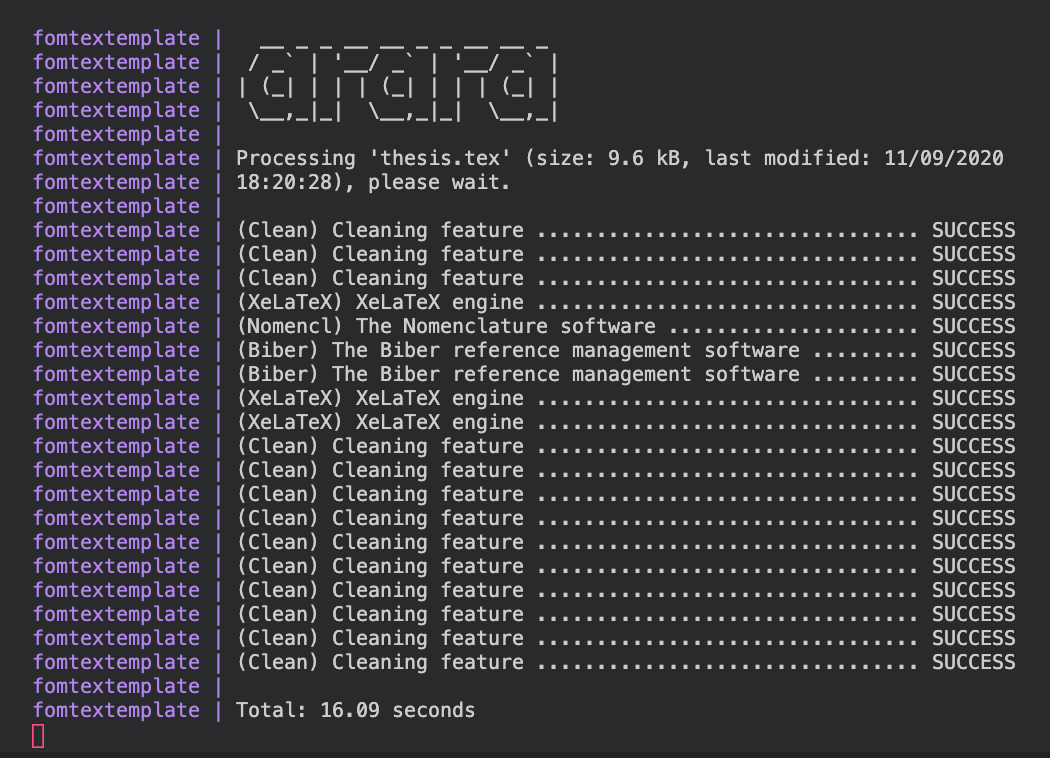
\includegraphics[width=1\textwidth]{.github/terminal}
    \captionsetup{width=1\textwidth}
    \capquelle{\cite[][200]{bsp}}\label{abb_bsp}
\end{figure}
\blindtext\footcite[Vgl. ][415-426]{Tanenbaum2016}

\subsubsection{Design-Prinzip der Separierung von Verantwortlichkeiten}
\blindtext\footcite[Vgl. ][79]{Schelinski2019}
\blinditemize
\Blindtext\footcite[Vgl. ][34]{Digitaloekonomie}

\section{Schluss}
\subsection{Fazit}
\Blindtext


qqw
12
22
2
1